\documentclass[aspectratio=169,10pt]{beamer}

\usepackage[T1]{fontenc}
\usepackage[utf8]{inputenc}
\usepackage{libertinus}
\usepackage{amsmath,amssymb}
\usepackage{graphicx}
\usepackage{booktabs}
\usepackage{ragged2e}
\usepackage{tikz}
\usetikzlibrary{arrows.meta,positioning,fit,calc}

\definecolor{DeckBg}{HTML}{FBF4EA}
\definecolor{DeckInk}{HTML}{172033}
\definecolor{DeckMuted}{HTML}{5B667A}
\definecolor{DeckLine}{HTML}{D9CDBB}
\definecolor{DeckBlue}{HTML}{1D4ED8}
\definecolor{DeckRust}{HTML}{B45309}
\definecolor{DeckSoft}{HTML}{F6EBDD}
\definecolor{DeckSand}{HTML}{F7EFE3}

\setbeamercolor{background canvas}{bg=DeckBg}
\setbeamercolor{normal text}{fg=DeckInk,bg=DeckBg}
\setbeamercolor{frametitle}{fg=DeckInk,bg=DeckBg}
\setbeamercolor{title}{fg=DeckInk}
\setbeamercolor{subtitle}{fg=DeckMuted}
\setbeamercolor{structure}{fg=DeckBlue}
\setbeamercolor{item}{fg=DeckBlue}
\setbeamercolor{block title}{fg=DeckInk,bg=DeckSoft}
\setbeamercolor{block body}{fg=DeckInk,bg=white}
\setbeamercolor{author in head/foot}{fg=DeckMuted,bg=DeckBg}

\usefonttheme{professionalfonts}
\setbeamertemplate{navigation symbols}{}
\setbeamertemplate{itemize item}{\color{DeckBlue}\raise0.2ex\hbox{\scriptsize\textbullet}}
\setbeamertemplate{itemize subitem}{\color{DeckBlue}\raise0.15ex\hbox{\tiny\textbullet}}
\setbeamertemplate{blocks}[rounded][shadow=false]
\setbeamerfont{title}{size=\fontsize{20}{24}\selectfont,series=\bfseries}
\setbeamerfont{subtitle}{size=\small}
\setbeamerfont{frametitle}{size=\fontsize{16.5}{20}\selectfont,series=\bfseries}
\setbeamerfont{block title}{size=\small,series=\bfseries}
\setbeamerfont{block body}{size=\small}

\setbeamertemplate{frametitle}{
  \vspace{0.1em}
  \insertframetitle
  \vspace{0.28em}
  \hrule height 0.3pt
}

\setbeamertemplate{footline}{
  \leavevmode
  \begin{beamercolorbox}[wd=\paperwidth,ht=2.8ex,dp=1.2ex,leftskip=1em,rightskip=1em]{author in head/foot}
    \tiny What Should Economics Ask Next? \hfill \insertframenumber/\inserttotalframenumber
  \end{beamercolorbox}
}

\newcommand{\takeaway}[1]{%
  \vspace{0.2em}
  {\footnotesize\color{DeckMuted}\parbox{0.9\linewidth}{\raggedright\textbullet\ #1}\par}
}

\newcommand{\figone}{%
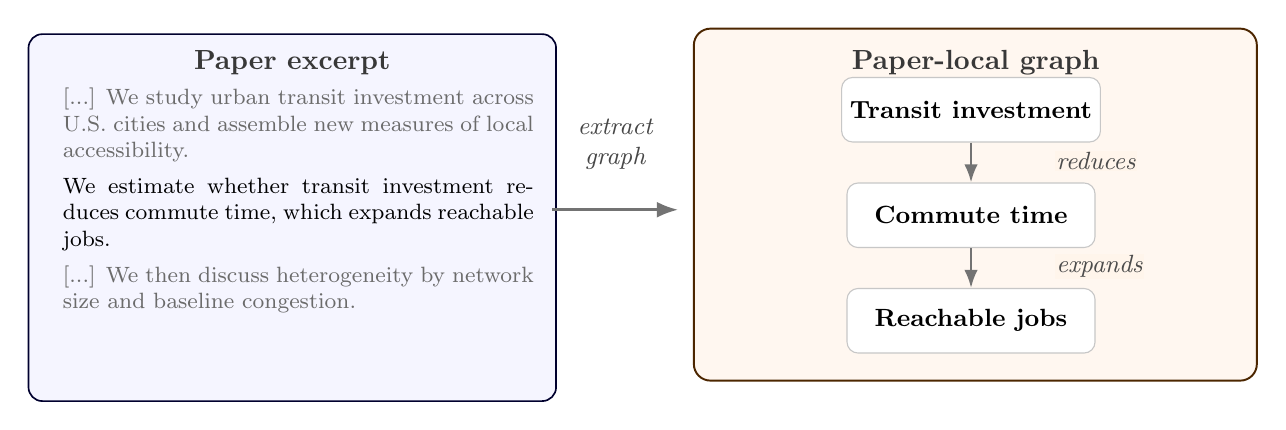
\begin{tikzpicture}[
  x=1cm, y=1cm,
  paperpanel/.style={draw=blue!18!black, rounded corners=5pt, fill=blue!4, line width=0.6pt},
  graphpanel/.style={draw=orange!30!black, rounded corners=6pt, fill=orange!6, line width=0.7pt},
  paneltitle/.style={font=\normalsize\bfseries, text=black!78},
  excerpt/.style={font=\footnotesize, align=justify, text width=5.98cm, inner sep=0pt},
  flownote/.style={font=\small\itshape, text=black!72},
  concept/.style={draw=black!22, rounded corners=4pt, fill=white, minimum width=3.15cm, minimum height=0.82cm, inner sep=3pt, font=\small\bfseries, align=center},
  relabel/.style={font=\small\itshape, text=black!70, fill=orange!10, fill opacity=0.38, text opacity=1, inner sep=0.45pt},
  flow/.style={-{Latex[length=2.7mm]}, draw=black!55, line width=1pt},
  edge/.style={-{Latex[length=2.3mm]}, draw=black!55, line width=0.9pt}
]
  \draw[paperpanel] (-0.25,-0.28) rectangle (6.45,4.38);
  \node[paneltitle] at (3.1,4.02) {Paper excerpt};
  \node[excerpt, anchor=north west] at (0.18,3.7) {%
    \textcolor{black!58}{[...] We study urban transit investment across U.S. cities and assemble new measures of local accessibility.}\par
    \vspace{0.42em}
    We estimate whether transit investment reduces commute time, which expands reachable jobs.\par
    \vspace{0.42em}
    \textcolor{black!58}{[...] We then discuss heterogeneity by network size and baseline congestion.}%
  };

  \draw[flow] (6.4,2.15) -- (8.0,2.15);
  \node[flownote, align=center] at (7.2,2.98) {extract\\graph};

  \draw[graphpanel] (8.2,-0.02) rectangle (15.35,4.45);
  \node[paneltitle] at (11.78,4.02) {Paper-local graph};

  \node[concept] (n1) at (11.72,3.42) {Transit investment};
  \node[concept] (n2) at (11.72,2.08) {Commute time};
  \node[concept] (n3) at (11.72,0.74) {Reachable jobs};

  \draw[edge] (n1) -- (n2);
  \draw[edge] (n2) -- (n3);
  \node[relabel, anchor=west] at (12.78,2.77) {reduces};
  \node[relabel, anchor=west] at (12.78,1.43) {expands};
\end{tikzpicture}%
}

\newcommand{\figtwo}{%
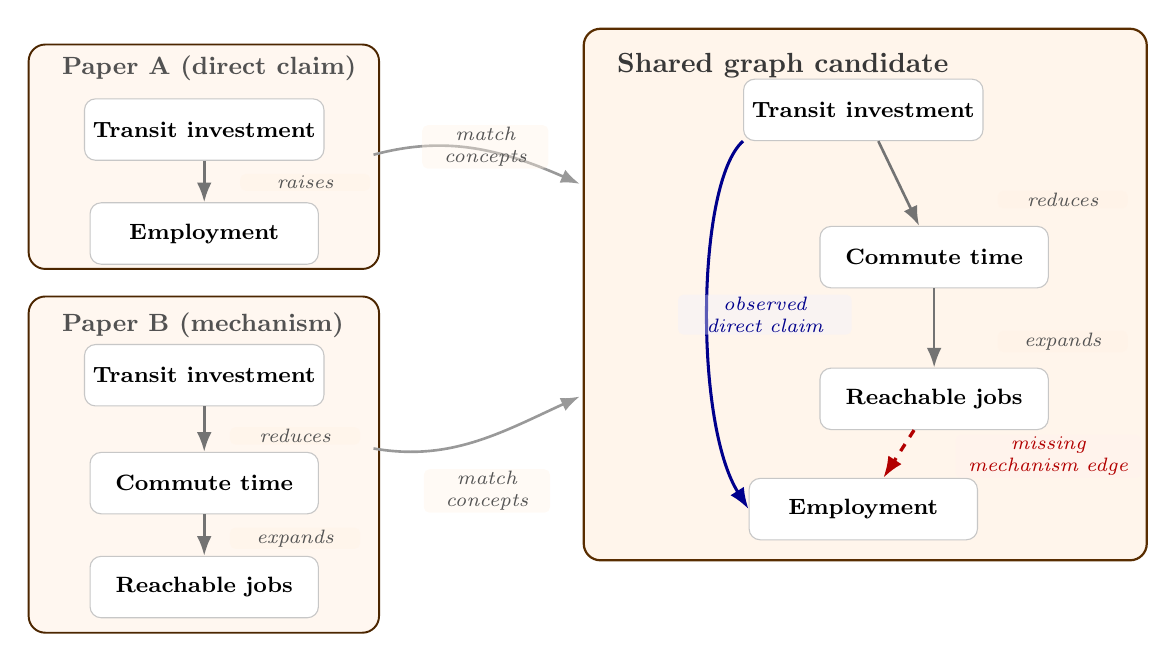
\begin{tikzpicture}[
  x=1cm, y=1cm,
  paperpanel/.style={draw=orange!30!black, rounded corners=6pt, fill=orange!6, line width=0.7pt},
  graphpanel/.style={draw=orange!35!black, rounded corners=6pt, fill=orange!8, line width=0.8pt},
  panelhead/.style={font=\normalsize\bfseries, text=black!78},
  paperhead/.style={font=\small\bfseries, text=black!68},
  concept/.style={draw=black!22, rounded corners=4pt, fill=white, minimum width=2.9cm, minimum height=0.78cm, inner sep=3pt, font=\footnotesize\bfseries, align=center},
  causal/.style={-{Latex[length=2.5mm]}, draw=black!55, line width=0.95pt},
  directclaim/.style={-{Latex[length=2.7mm]}, draw=blue!55!black, line width=1.1pt},
  missedge/.style={-{Latex[length=2.7mm]}, draw=red!70!black, line width=1.2pt, dashed},
  matcher/.style={-{Latex[length=2.4mm]}, draw=black!40, line width=0.95pt},
  edgelabel/.style={font=\scriptsize\itshape, text=black!67, fill=orange!10, fill opacity=0.38, text opacity=1, rounded corners=2pt, inner sep=0.75pt, align=center, text width=1.6cm},
  bluelabel/.style={font=\scriptsize\itshape, text=blue!55!black, fill=blue!6, fill opacity=0.38, text opacity=1, rounded corners=2pt, inner sep=0.8pt, align=center, text width=2.15cm},
  redlabel/.style={font=\scriptsize\itshape, text=red!70!black, fill=red!6, fill opacity=0.38, text opacity=1, rounded corners=2pt, inner sep=0.8pt, align=center, text width=2.3cm}
]
  \draw[paperpanel] (0,3.9) rectangle (4.45,6.75);
  \node[paperhead, anchor=west] at (0.3,6.45) {Paper A (direct claim)};
  \node[concept] (a1) at (2.23,5.67) {Transit investment};
  \node[concept] (a2) at (2.23,4.35) {Employment};
  \draw[causal] (a1) -- (a2);
  \node[edgelabel, anchor=west] at (2.68,5.0) {raises};

  \draw[paperpanel] (0,-0.72) rectangle (4.45,3.55);
  \node[paperhead, anchor=west] at (0.3,3.18) {Paper B (mechanism)};
  \node[concept] (b1) at (2.23,2.55) {Transit investment};
  \node[concept] (b2) at (2.23,1.18) {Commute time};
  \node[concept] (b3) at (2.23,-0.14) {Reachable jobs};
  \draw[causal] (b1) -- (b2);
  \draw[causal] (b2) -- (b3);
  \node[edgelabel, anchor=west] at (2.55,1.78) {reduces};
  \node[edgelabel, anchor=west] at (2.55,0.48) {expands};

  \draw[matcher] (4.38,5.35) .. controls (5.3,5.6) and (6.0,5.42) .. (7.0,4.98);
  \draw[matcher] (4.38,1.62) .. controls (5.35,1.45) and (6.0,1.82) .. (7.0,2.28);
  \node[edgelabel, text width=1.55cm] at (5.8,5.45) {match concepts};
  \node[edgelabel, text width=1.55cm] at (5.82,1.08) {match concepts};

  \draw[graphpanel] (7.05,0.2) rectangle (14.2,6.95);
  \node[panelhead, anchor=west] at (7.35,6.48) {Shared graph candidate};

  \node[concept] (g1) at (10.6,5.92) {Transit investment};
  \node[concept] (g2) at (11.5,4.05) {Commute time};
  \node[concept] (g3) at (11.5,2.25) {Reachable jobs};
  \node[concept] (g4) at (10.6,0.85) {Employment};

  \draw[causal] (g1) -- (g2);
  \draw[causal] (g2) -- (g3);
  \draw[directclaim] (g1.south west) .. controls (8.48,5.0) and (8.45,1.95) .. (g4.west);
  \draw[missedge] (g3) -- (g4);

  \node[edgelabel, anchor=west] at (12.3,4.78) {reduces};
  \node[edgelabel, anchor=west] at (12.3,2.98) {expands};
  \node[bluelabel] at (9.35,3.32) {observed\\direct claim};
  \node[redlabel] at (12.95,1.52) {missing\\mechanism edge};
\end{tikzpicture}%
}

\newcommand{\figfour}{%
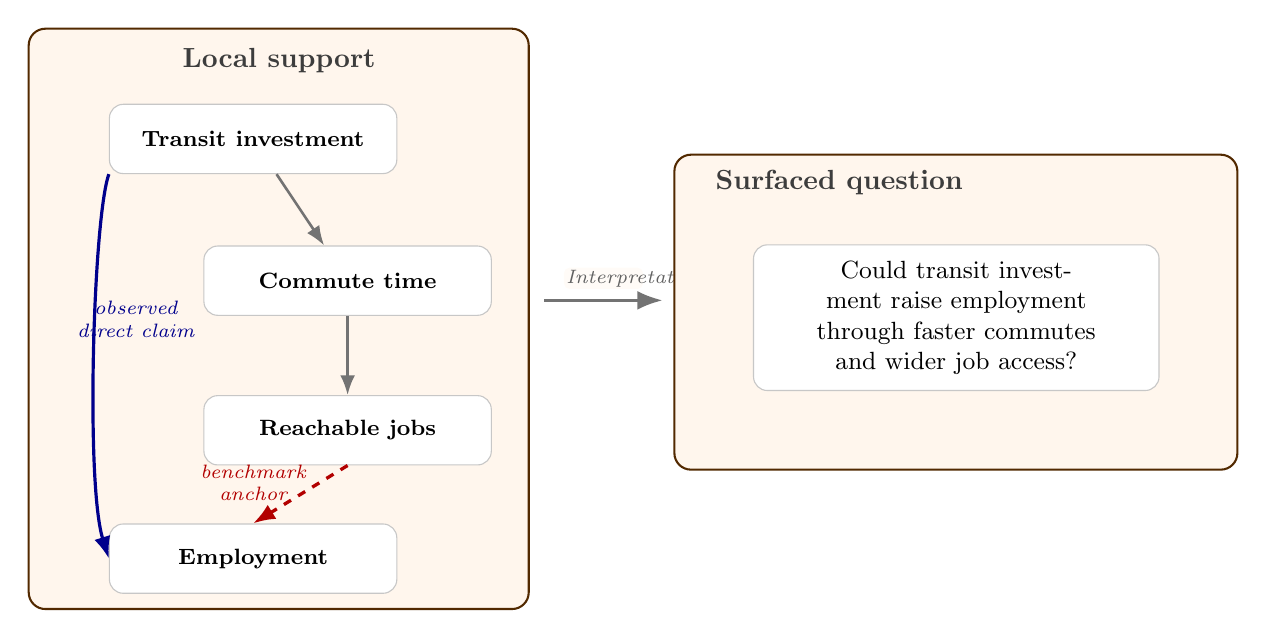
\begin{tikzpicture}[
  x=1cm,y=1cm,
  panel/.style={draw=orange!32!black, rounded corners=6pt, fill=orange!7, line width=0.75pt},
  panelhead/.style={font=\normalsize\bfseries, text=black!76},
  concept/.style={draw=black!22, rounded corners=5pt, fill=white, minimum width=3.65cm, minimum height=0.88cm, inner sep=3pt, font=\footnotesize\bfseries, align=center},
  qbox/.style={draw=black!22, rounded corners=5pt, fill=white, minimum width=5.15cm, minimum height=1.85cm, inner sep=5pt, font=\small, align=center, text width=4.55cm},
  causal/.style={-{Latex[length=2.5mm]}, draw=black!55, line width=0.95pt},
  directclaim/.style={-{Latex[length=2.8mm]}, draw=blue!55!black, line width=1.15pt},
  missedge/.style={-{Latex[length=2.8mm]}, draw=red!70!black, line width=1.2pt, dashed},
  compress/.style={-{Latex[length=3.2mm]}, draw=black!55, line width=1.05pt},
  blabel/.style={font=\scriptsize\itshape, text=blue!55!black, align=center},
  rlabel/.style={font=\scriptsize\itshape, text=red!70!black, align=center},
  flowlabel/.style={font=\scriptsize\itshape, text=black!62, fill=orange!8, fill opacity=0.38, text opacity=1, rounded corners=2pt, inner sep=0.8pt, align=center, text width=0.95cm}
]
  \draw[panel] (0,-0.82) rectangle (6.35,6.55);
  \node[panelhead] at (3.18,6.15) {Local support};

  \node[concept] (l1) at (2.85,5.15) {Transit investment};
  \node[concept] (l2) at (4.05,3.35) {Commute time};
  \node[concept] (l3) at (4.05,1.45) {Reachable jobs};
  \node[concept] (l4) at (2.85,-0.18) {Employment};

  \draw[causal] (l1) -- (l2);
  \draw[causal] (l2) -- (l3);
  \draw[directclaim] (l1.south west) .. controls (0.82,4.15) and (0.72,0.78) .. (l4.west);
  \draw[missedge] (l3.south) -- (l4.north);

  \node[blabel] at (1.36,2.86) {observed\\direct claim};
  \node[rlabel] at (2.85,0.78) {benchmark\\anchor};

  \draw[compress] (6.55,3.1) -- (8.05,3.1);
  \node[flowlabel] at (7.3,3.38) {Interpretation};

  \draw[panel] (8.2,0.95) rectangle (15.35,4.95);
  \node[panelhead, anchor=west] at (8.6,4.6) {Surfaced question};
  \node[qbox] at (11.78,2.88) {Could transit investment raise employment\\
  through faster commutes\\
  and wider job access?};
\end{tikzpicture}%
}

\newcommand{\figsixslide}{%
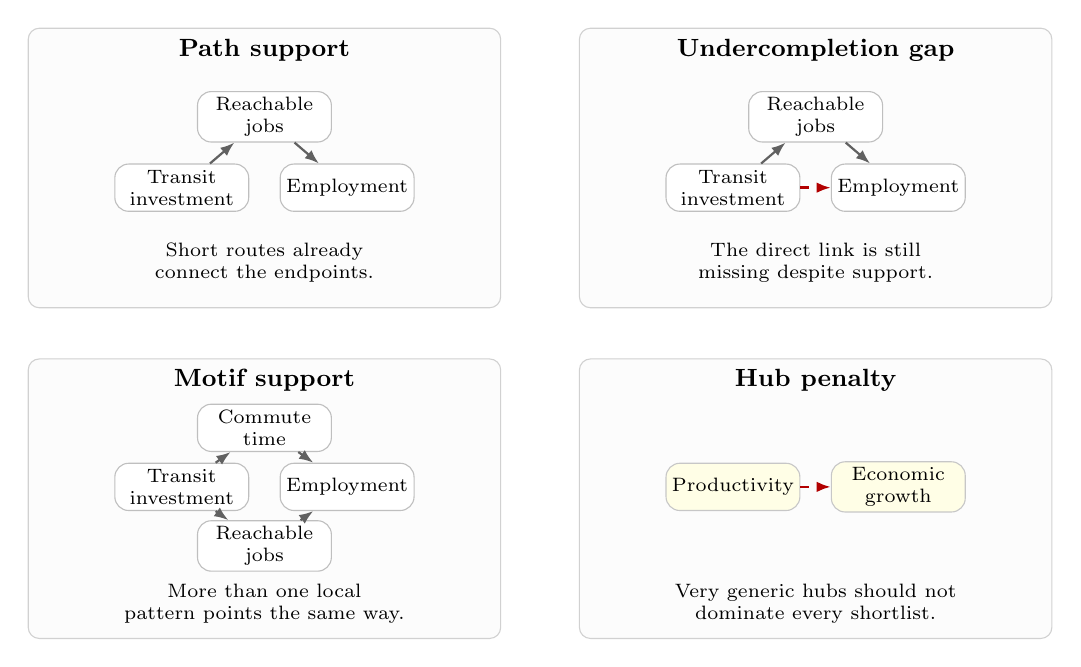
\begin{tikzpicture}[
  x=1cm,y=1cm,
  panel/.style={draw=black!18, rounded corners=4pt, fill=gray!2, minimum width=6.0cm, minimum height=3.55cm},
  node/.style={draw=black!25, rounded corners=5pt, fill=white, minimum width=1.7cm, minimum height=0.6cm, inner sep=2pt, font=\scriptsize, align=center},
  hub/.style={draw=black!22, rounded corners=5pt, fill=yellow!10, minimum width=1.7cm, minimum height=0.6cm, inner sep=2pt, font=\scriptsize, align=center},
  edge/.style={-{Latex[length=1.8mm]}, draw=black!62, line width=0.8pt},
  miss/.style={-{Latex[length=1.8mm]}, draw=red!70!black, dashed, line width=0.95pt},
  lab/.style={font=\small\bfseries}
]
  \node[panel] at (3.5,4.35) {};
  \node[panel] at (10.5,4.35) {};
  \node[panel] at (3.5,0.15) {};
  \node[panel] at (10.5,0.15) {};
  \node[lab] at (3.5,5.85) {Path support};
  \node[lab] at (10.5,5.85) {Undercompletion gap};
  \node[lab] at (3.5,1.65) {Motif support};
  \node[lab] at (10.5,1.65) {Hub penalty};

  \node[node] (k1) at (2.45,4.1) {Transit\\investment};
  \node[node] (k2) at (3.5,5.0) {Reachable\\jobs};
  \node[node] (k3) at (4.55,4.1) {Employment};
  \draw[edge] (k1) -- (k2);
  \draw[edge] (k2) -- (k3);
  \node[font=\scriptsize, align=center] at (3.5,3.15) {Short routes already\\connect the endpoints.};

  \node[node] (l1) at (9.45,4.1) {Transit\\investment};
  \node[node] (l2) at (10.5,5.0) {Reachable\\jobs};
  \node[node] (l3) at (11.55,4.1) {Employment};
  \draw[edge] (l1) -- (l2);
  \draw[edge] (l2) -- (l3);
  \draw[miss] (l1) -- (l3);
  \node[font=\scriptsize, align=center] at (10.5,3.15) {The direct link is still\\missing despite support.};

  \node[node] (m1) at (2.45,0.3) {Transit\\investment};
  \node[node] (m2) at (3.5,1.05) {Commute\\time};
  \node[node] (m3) at (3.5,-0.45) {Reachable\\jobs};
  \node[node] (m4) at (4.55,0.3) {Employment};
  \draw[edge] (m1) -- (m2);
  \draw[edge] (m2) -- (m4);
  \draw[edge] (m1) -- (m3);
  \draw[edge] (m3) -- (m4);
  \node[font=\scriptsize, align=center] at (3.5,-1.18) {More than one local\\pattern points the same way.};

  \node[hub] (n1) at (9.45,0.3) {Productivity};
  \node[hub] (n2) at (11.55,0.3) {Economic\\growth};
  \draw[miss] (n1) -- (n2);
  \node[font=\scriptsize, align=center] at (10.5,-1.18) {Very generic hubs should not\\dominate every shortlist.};
\end{tikzpicture}%
}

\title{What Should Economics Ask Next?}
\author{Prashant Garg \\ Imperial College London}
\date{April 2026}

\begin{document}

\begin{frame}[plain]
  \titlepage
  \vspace{-1.2em}
  \begin{center}
    {\small\color{DeckMuted}Project site: \href{https://frontiergraph.com}{\textcolor{DeckBlue}{frontiergraph.com}}}
  \end{center}
\end{frame}

\begin{frame}{Why this problem?}
\begin{columns}[T,totalwidth=0.95\textwidth]
\column{0.46\textwidth}
\vspace{0.2em}
{\Large\bfseries
Question choice is still the weakly formalized part of research.
}

\vspace{0.85em}
{\small
\begin{itemize}
  \item We have better tools for analyzing a paper than for deciding what to work on next.
  \item The problem gets sharper as the literature grows and local reading becomes harder.
\end{itemize}
}

\column{0.46\textwidth}
\begin{block}{Why now}
{\small
\textbf{Scale.} The published literature is large, path dependent, and hard to scan locally.
}
\end{block}

\vspace{0.45em}
\setbeamercolor{block title}{fg=DeckInk,bg=blue!12}
\setbeamercolor{block body}{fg=DeckInk,bg=white}
\begin{block}{Why the graph helps}
{\small
\textbf{Structure.} Nearby paths and repeated concepts make open questions more inspectable.
}
\end{block}

\vspace{0.45em}
\setbeamercolor{block title}{fg=DeckInk,bg=orange!18}
\setbeamercolor{block body}{fg=DeckInk,bg=white}
\begin{block}{Why the timing matters}
{\small
\textbf{AI shift.} If downstream tasks get cheaper, the bottleneck moves upstream toward question choice.
}
\end{block}
\end{columns}
\setbeamercolor{block title}{fg=DeckInk,bg=DeckSoft}
\setbeamercolor{block body}{fg=DeckInk,bg=white}
\end{frame}

\begin{frame}{Where this sits in the literature}
\begin{columns}[T,totalwidth=0.95\textwidth]
\column{0.48\textwidth}
\begin{block}{Adjacent literatures}
{\small
\begin{itemize}
  \item \textbf{Economics of ideas.} Bloom et al.\ on ideas getting harder to find; Jones on the knowledge burden; Azoulay, Graff Zivin, and Manso on incentives for exploration.
  \item \textbf{Science of science.} Fortunato et al.\ and Wang--Barab\'asi on frontier formation, novelty, and cumulative attention.
  \item \textbf{Knowledge-graph discovery.} Rzhetsky et al., Sourati et al., Tong et al., and Lee et al.\ on missing links as candidate discoveries.
\end{itemize}
}
\end{block}

\column{0.44\textwidth}
\begin{block}{What this paper adds}
{\small
\begin{itemize}
  \item A \textbf{directed economics claim graph} rather than a generic scientific graph.
  \item Two \textbf{historical question objects} that can be backtested prospectively.
  \item A comparison between \textbf{popularity, local structure, and learned reranking} on the same candidate set.
  \item An \textbf{economics-facing use case}: screening scarce reading time and early project choice.
\end{itemize}
}
\end{block}
\end{columns}
\takeaway{The contribution is not a new foundation model. It is a benchmarkable graph object for choosing what to inspect next.}
\end{frame}

\begin{frame}{Each paper first becomes a local graph}
\centering
{\scriptsize
\parbox{0.94\linewidth}{\raggedright
\textbullet\ \textbf{Model}: GPT-5.4-mini. \textbf{Papers}: 242K papers (1976--2026) from top 150 economics journals and econ papers in top 150 adjacent journals. \textbf{Source}: OpenAlex.\\[0.2em]
Method follows Garg and Fetzer (2025), \href{https://www.causal.claims/}{\emph{Causal Claims in Economics}}.
}}
\vspace{0.35em}
\centering
\resizebox{!}{0.5\textheight}{\figone}
\end{frame}

\begin{frame}{An ontology to match nodes across papers}
\begin{columns}[T,totalwidth=0.94\textwidth]
\column{0.45\textwidth}
\begin{block}{Ontology sources}
{\scriptsize
\begin{itemize}
  \setlength{\itemsep}{0.1em}
  \item JEL (5,001 nodes)
  \item Wikidata (8,383 nodes)
  \item OpenAlex topics (1,876 nodes)
  \item OpenAlex keywords (9,271 nodes)
  \item Economics-filtered Wikipedia (129,032 nodes)
\end{itemize}
}
\end{block}

\vspace{0.2em}
\begin{block}{Scale}
{\scriptsize
\textbf{Frozen baseline}: 154,359 ontology rows.\\[0.2em]
\textbf{Benchmark graph}: 230,479 papers and 1,271,014 normalized links.
}
\end{block}

\column{0.45\textwidth}
\begin{block}{Grounding logic}
{\scriptsize
\textbf{Stage 1.} Exact label, surface-form, and stripped-parenthesis matches.\\[0.25em]
\textbf{Stage 2.} Semantic embedding retrieval, with rank-1 to rank-3 candidates stored for audit.\\[0.25em]
\textbf{Principle.} Use embeddings as retrieval after easy cases are solved, not as an unconstrained merge rule.
}
\end{block}

\vspace{0.1em}
\begin{block}{Why this matters}
{\scriptsize
\begin{itemize}
  \setlength{\itemsep}{0.1em}
  \item Candidate generation only works if repeated labels map to stable concepts.
  \item Path counts and missing links move mechanically when identity is noisy.
  \item Conservative merging is better than fake novelty created by label variation.
  \item Uncertain cases stay visible for audit instead of being hidden.
\end{itemize}
}
\end{block}
\end{columns}
\end{frame}

\begin{frame}{Cross-paper matching creates the shared candidate neighborhood}
\centering
{\scriptsize
\parbox{0.94\linewidth}{\raggedright
Repeated concepts are then matched across papers, so paper-local edges can become shared candidate neighborhoods.
}}
\vspace{0.35em}
\centering
\resizebox{!}{0.52\textheight}{\figtwo}
\end{frame}

\begin{frame}{Two historical question objects}
\centering
{\scriptsize
\parbox{0.94\linewidth}{\centering
The graph matures in two distinct ways over time: it can add a missing direct link, or deepen an existing claim with a clearer mechanism.
}}
\vspace{0.45em}
\begin{columns}[T,totalwidth=0.94\textwidth]
\column{0.45\textwidth}
\begin{block}{Direct-to-path}
\begin{itemize}
  \item A direct relation is already in the literature.
  \item Later work adds a clearer mechanism around it.
  \item This is the mechanism-thickening object.
\end{itemize}
\end{block}

\column{0.45\textwidth}
\begin{block}{Path-to-direct}
\begin{itemize}
  \item Nearby support already exists.
  \item The direct relation itself is still missing.
  \item Later work states that direct link explicitly.
\end{itemize}
\end{block}
\end{columns}
\end{frame}

\begin{frame}{Setting historical benchmark}
\centering
\vspace{0.2em}
\begin{columns}[T,totalwidth=0.95\textwidth]
\column{0.30\textwidth}
\begin{block}{1. Candidate set}
\begin{itemize}
  \item Freeze the graph at date \(t-1\).
  \item Collect still-open pairs implied by local support neighborhoods.
\end{itemize}
\end{block}

\column{0.30\textwidth}
\begin{block}{2. Ranking rule}
\begin{itemize}
  \item Order same candidates in three ways:
  \begin{itemize}
    \item popularity (preferential attachment)
    \item local graph structure
    \item local graph structure + learned refinement
  \end{itemize}
\end{itemize}
\end{block}

\column{0.30\textwidth}
\begin{block}{3. Historical check}
\begin{itemize}
  \item Set horizon \(h \in \{5,10,15\}\) years.
  \item Check which ranked questions later appear in published work.
\end{itemize}
\end{block}
\end{columns}
\end{frame}

\begin{frame}{Three ways to rank the same open questions}
\centering
{\scriptsize
\parbox{0.94\linewidth}{\centering
Hold the candidate set fixed. Change only the ordering rule.
}}
\vspace{0.45em}
\begin{columns}[T,totalwidth=0.95\textwidth]
\column{0.29\textwidth}
\begin{block}{Popularity baseline}
\begin{itemize}
  \item High-degree endpoints rise first.
  \item Tests whether visibility alone explains later uptake.
  \item Statistic: endpoint degree and centrality only.
\end{itemize}
\end{block}

\column{0.29\textwidth}
\begin{block}{Structural score}
\begin{itemize}
  \item A hand-set score on local graph structure.
  \item Rewards supported but still incomplete pairs.
  \item Components: motif support, undercompletion gap, and hub penalty.
\end{itemize}
\end{block}

\column{0.29\textwidth}
\begin{block}{Learned reranker}
\begin{itemize}
  \item A supervised model on the same candidate set.
  \item Tests whether richer features improve on the structural score.
  \item Trained in walk-forward windows on 34 graph-derived features and later edge appearance.
\end{itemize}
\end{block}
\end{columns}
\takeaway{The comparison is centrality vs structure vs supervised refinement.}
\end{frame}

\begin{frame}{What the structural score rewards}
\centering
\resizebox{0.86\linewidth}{!}{\figsixslide}
\end{frame}

\begin{frame}{Graph screening beats popularity in historical shortlists}
\centering
\centering
\includegraphics[width=0.59\linewidth]{../outputs/paper/149_dual_family_main_pairing/dual_family_main_benchmark.pdf}
\takeaway{Direct-to-path gives denser shortlists. Path-to-direct covers more of the later-realized links.}
\end{frame}

\begin{frame}{Historical uptake favors mechanism thickening over direct closure}
\centering
\vspace{0.1em}
\centering

\includegraphics[width=0.74\linewidth]{../outputs/paper/138_path_evolution_refresh/figures/path_evolution_comparison.png}

\takeaway{Economics more often thickens mechanisms around existing claims than later closes locally implied direct links.}
\end{frame}

\begin{frame}{The current frontier looks like a set of readable mechanism questions}
\centering
\includegraphics[width=0.85\linewidth]{../outputs/paper/154_dual_family_extension_pairing/dual_family_current_frontier_summary.pdf}
\end{frame}

\begin{frame}{Most realizing papers take up one predicted edge}
\begin{block}{Bundle uptake}
\begin{itemize}
  \item About 95\% of realizing papers take up exactly one predicted edge.
  \item Mixed-family bundles are rare, around 0.1--0.2\% of realizing papers.
  \item When multiple predicted edges appear in one paper, they stay local in graph space rather than spanning unrelated mechanisms.
\end{itemize}
\end{block}
\vspace{0.5em}
\begin{block}{Interpretation}
\begin{itemize}
  \item The surfaced object usually maps to one concrete extension, not a diffuse shopping list.
  \item That makes the shortlist easier to read as a screening tool for actual project formation.
\end{itemize}
\end{block}
\end{frame}

\begin{frame}{Path-to-direct is taken up by larger, more funded teams}
\begin{columns}[T,totalwidth=0.95\textwidth]
\column{0.60\textwidth}
\centering
\includegraphics[width=\linewidth]{../outputs/paper/181_slides_followon_results/adopter_profile_coef_only.pdf}

\column{0.33\textwidth}
\begin{block}{At \(h=10\)}
\begin{itemize}
  \item Team size: \(2.86\) vs \(2.39\)
  \item Funding: \(18.5\%\) vs \(5.4\%\)
  \item Cross-country: \(30.0\%\) vs \(20.4\%\)
  \item Career age: younger teams on average
\end{itemize}
\end{block}
\end{columns}
\vspace{0.45em}
\takeaway{Path-to-direct is taken up by more resourced and more collaborative teams, suggesting that closing a missing direct link is the narrower and more demanding motion.}
\end{frame}

\begin{frame}{Conclusion}
\begin{columns}[T,totalwidth=0.95\textwidth]
\column{0.30\textwidth}
\begin{block}{What we built}
{\small
\begin{itemize}
  \item Claim graph from 242K economics-facing papers.
  \item Cross-paper ontology matching plus dated local neighborhoods.
  \item Two historical question objects with walk-forward evaluation.
\end{itemize}
}
\end{block}

\column{0.30\textwidth}
\begin{block}{What we found}
{\small
\begin{itemize}
  \item Structural screening beats a popularity baseline in historical shortlists.
  \item Learned reranking improves further on the same candidate set.
  \item Economics more often deepens mechanisms than closes missing direct links.
\end{itemize}
}
\end{block}

\column{0.30\textwidth}
\begin{block}{What to take from it}
{\small
\begin{itemize}
  \item A prototype for AI-assisted question choice, not research autopilot.
  \item Best used to focus reading, inspection, and early project formation.
  \item Useful when the bottleneck shifts upstream from execution to question choice.
\end{itemize}
}
\end{block}
\end{columns}

\vspace{0.65em}
\begin{center}
{\small\color{DeckMuted}\href{https://frontiergraph.com}{\textcolor{DeckBlue}{frontiergraph.com}}: visit for frontier ideas, data, code, and the full graph explorer}
\end{center}
\end{frame}

\begin{frame}{References}
\scriptsize
\begin{columns}[T,totalwidth=0.97\textwidth]
\column{0.48\textwidth}
\begin{itemize}
  \item Agrawal, McHale, and Oettl (2024), ``AI and the economics of prioritized search.''
  \item Azoulay, Graff Zivin, and Manso (2011), ``Incentives and creativity.''
  \item Barab\'asi and Albert (1999), ``Emergence of scaling in random networks.''
  \item Bloom, Jones, Van Reenen, and Webb (2020), ``Are ideas getting harder to find?''
  \item Fortunato et al. (2018), ``Science of science.''
  \item Foster, Rzhetsky, and Evans (2015), ``Tradition and innovation in scientists' research strategies.''
  \item Garg and Fetzer (2025), ``Causal Claims in Economics.''
  \item Jones (2009), ``The burden of knowledge and the death of the renaissance man.''
\end{itemize}

\column{0.48\textwidth}
\begin{itemize}
  \item Lee et al. (2024), ``EconCausal: a benchmark for causal reasoning in economics and finance.''
  \item Liu (2009), \emph{Learning to Rank for Information Retrieval.}
  \item Rzhetsky et al. (2015), ``Choosing experiments to accelerate collective discovery.''
  \item Sourati et al. (2023), ``Accelerating science with human-aware AI.''
  \item Tong et al. (2024), ``Automating the generation of scientific hypotheses from causal knowledge graphs.''
  \item Wang, Veugelers, and Stephan (2017), ``Bias against novelty in science.''
  \item Wang and Barab\'asi (2021), \emph{The Science of Science.}
\end{itemize}
\end{columns}
\end{frame}

\end{document}
